\documentclass{standalone}


% Copy of relevant parts from the main preamble.
\usepackage{mathtools}

% Uncomment the following to use Times New Roman and Cambria Math
% \usepackage{unicode-math}
% \unimathsetup{math-style=TeX}
% \setmathfont[range=\mathup/{num}]{Times New Roman}
% \setmathfont[range=\mathit/{greek,Greek,latin,Latin}]{Cambria Math}
% \setmathfont[range=\mathup/{greek,Greek,latin,Latin}]{Cambria Math}
% \setmathfont[range={"2212,"002B,"003D,"0028,"0029,"005B,"005D,"221A,
% "2211,"2248,"222B,"007C,"2026,"2202,"00D7,"0302,"2261,"0025,"22C5,
% "00B1,"2194,"21D4,"2032}]
% {Cambria Math}
% \setmainfont[Ligatures=TeX]{Times New Roman}

% Uncomment the following to use Linux Libertine
% \usepackage[libertine]{newtxmath}
% \usepackage[no-math]{fontspec}
% \setmainfont{Linux Libertine O}

% Uncomment the following to use TeX Gyre Termes
% \usepackage{unicode-math}
% \unimathsetup{math-style=TeX}
% \setmainfont{TeX Gyre Termes}
% \setmathfont{TeX Gyre Termes Math}

% Uncomment the following to use TeX Gyre Pagella
\usepackage{unicode-math}
\unimathsetup{math-style=TeX}
\setmainfont{TeX Gyre Pagella}
\setmathfont{TeX Gyre Pagella Math}

% \usepackage[sfmath]{kpfonts}
% \renewcommand*\familydefault{\sfdefault}
% \usepackage[T1]{fontenc}

% \usepackage[no-math]{fontspec}
% Always use Inconsolata
\setmonofont{Inconsolata}

\usepackage{microtype}


\usepackage[version=3]{mhchem}
\usepackage{chemfig}
\setatomsep{2.25em}
\usetikzlibrary{positioning, calc, arrows.meta}
\tikzset{
    flux/.style={
        flux/.cd,
        #1,
        print,
    },
    flux/.cd,
    position/.store in=\position,
    position=0.4,
    fluxabove/.store in=\fluxabove,
    fluxbelow/.store in=\fluxbelow,
    print/.style={
        /tikz/.cd,
        insert path={%
            node [pos=\position, above] {\SI{\fluxabove}{\percent}} node[pos=\position, below] {\textbf{\SI{\fluxbelow}{\percent}}}%
        },
    },
}
\usepackage{siunitx}
\sisetup{detect-all=true}

\begin{document}
    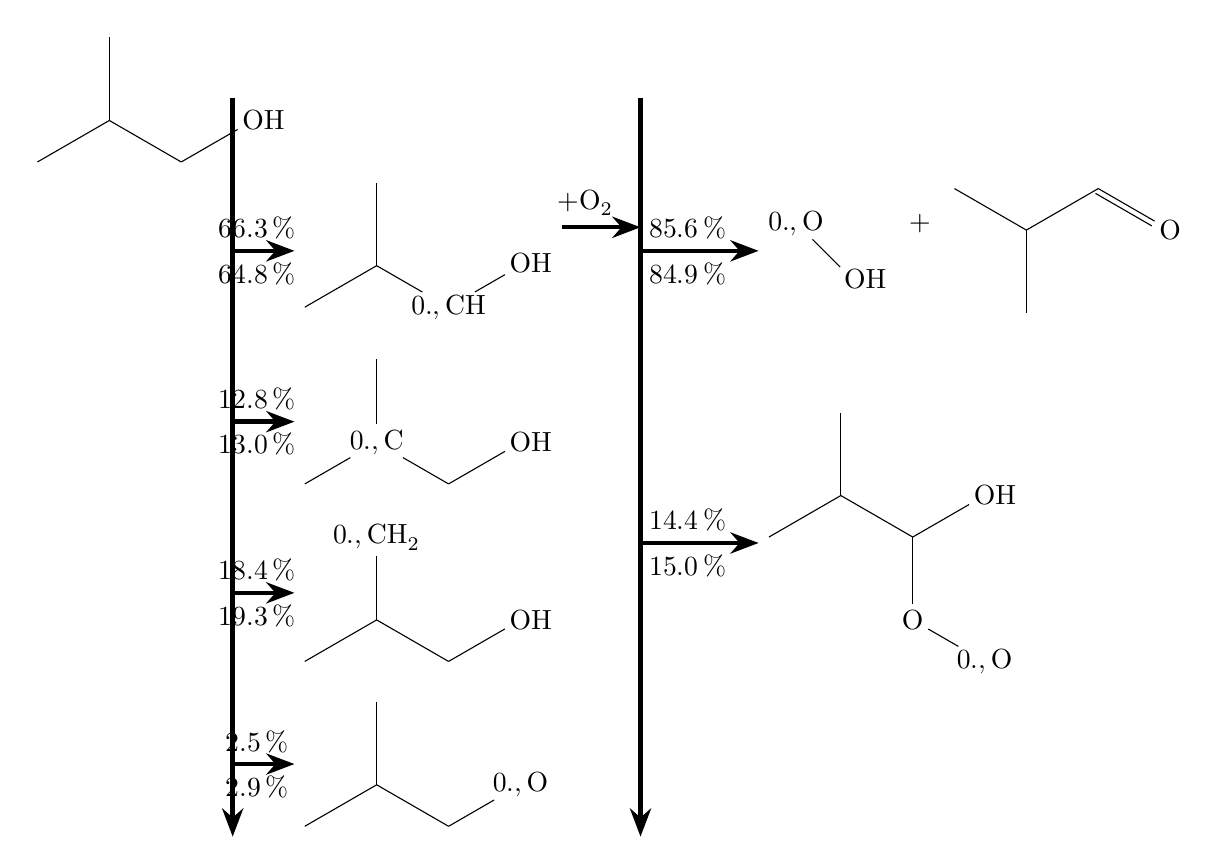
\begin{tikzpicture}[x=1cm, y=1cm, remember picture]
        \begin{scope}[every node/.style={node distance=0.25 and 0}]
            \node (ibuoh) {\chemfig{-[:30]@{midc}(-[2])-[:330]-[:30]OH}};
            \node[below right=0 and 0 of ibuoh] (aibuoh) {\chemfig{-[:30](-[2])-[:330]\lewis{0.,CH}-[:30]OH}};
            \node[below left=of aibuoh, anchor=north west] (bibuoh) {\chemfig{-[:30]\lewis{0.,C}(-[2])-[:330]-[:30]OH}};
            \node[below left=of bibuoh, anchor=north west] (gibuoh) {\chemfig{-[:30](-[2]\lewis{0.,CH_2})-[:330]-[:30]OH}};
            \node[below left=of gibuoh, anchor=north west] (oibuoh) {\chemfig{-[:30](-[2])-[:330]-[:30]\lewis{0.,O}}};
            \node[right=2.5 of aibuoh] (ibuohalde) {\chemfig{\lewis{0.,O}-[7]OH} \, $+$ \, \chemfig[baseline=(c)]{-[:330]@{c}(-[6])-[:30]=_[:330]O}};
            \node[below left=1 and 0 of ibuohalde, anchor=north west] (aibuohoo) {\chemfig{-[:30](-[2])-[:330](-[6]O-[:330]\lewis{0.,O})-[:30]OH}};
        \end{scope}

        \begin{scope}[every path/.style={draw, ultra thick, >={Stealth}}]
            \coordinate (linestart) at ($(midc)-(0,0.5)$);
            \path[->] let \p1 = (oibuoh.south), \p2 = (linestart) in (\x2,\y2) -- (\x2,\y1) coordinate (lineend);
            \path[->] ($(linestart)!(aibuoh)!(lineend)$) -- (aibuoh.west) [flux={fluxabove=66.3, fluxbelow=64.8}];
            \path[->] ($(linestart)!(bibuoh)!(lineend)$) -- (bibuoh.west) [flux={fluxabove=12.8, fluxbelow=13.0}];
            \path[->] ($(linestart)!(gibuoh)!(lineend)$) -- (gibuoh.west) [flux={fluxabove=18.4, fluxbelow=19.3}];
            \path[->] ($(linestart)!(oibuoh)!(lineend)$) -- (oibuoh.west) [flux={fluxabove=2.5, fluxbelow=2.9}];
            \coordinate (midline) at ($(aibuoh.east)!0.4!(ibuohalde.west)$);
            \path[->] let \p1 = (linestart), \p2 = (midline), \p3 = (lineend) in (\x2,\y1) -- (\x2,\y3) coordinate (midlineend);
            \path[->] (aibuoh.10) -- ($(midline)!(aibuoh.10)!(midlineend)$) node[above, pos=0.3] {$+$\ce{O2}};
            \path[->] ($(midline)!(ibuohalde)!(midlineend)$) -- (ibuohalde.west) [flux={fluxabove=85.6, fluxbelow=84.9}];
            \path[->] ($(midline)!(aibuohoo)!(midlineend)$) -- (aibuohoo.west) [flux={fluxabove=14.4, fluxbelow=15.0}];
        \end{scope}
    \end{tikzpicture}
\end{document}
